\documentclass[10pt,letterpaper]{article}

\usepackage[margin=0.75in]{geometry}
\usepackage{tikz}
\usepackage{graphicx}
\usepackage{amsmath}
\graphicspath{{img/}}
\begin{document}

  \title{Stats 314, Data Analysis \#3}
  \author{Cody Malick\\
  \texttt{malickc@oregonstate.edu}}
  \date{\today}
  \maketitle

\section*{Part I}
\subsection*{Scenario 1}
C. One sample t test\\
We want to use a one sample t test because we know the population average of 38
hours. Because we know the population average, we can compare the sample mean
with the population mean to make a decision as to whether or not the sample mean
if better or worse than the population mean.

\subsection*{Scenario 2}
D. Matched pairs t test
We have two sets of sample means, before and after, and we want to determine if
there was an improvement or not. This is perfect for a matched pair t test.

\subsection*{Scenario 3}
B. Two sample t test
The two sample t test is used to see if two sets of averages are equal, or if
one is better than the other. 

\subsection*{Scenario 4}
A. One sample z test for a mean
Given the information we have, we can see that the sample mean is relatively
close to the population mean, with a low standard deviation. This is usually
indictive of a normal distribution. But we want to use this test to see if a
given null hypothesis holds or is rejected. In this case, the null hypothesis
would be weight = 77 lbs. 

\section*{Part II}
\subsection*{a}
$\mu = 69.63938$\\
$\sigma = 4.066723$\\
The population is 256\\
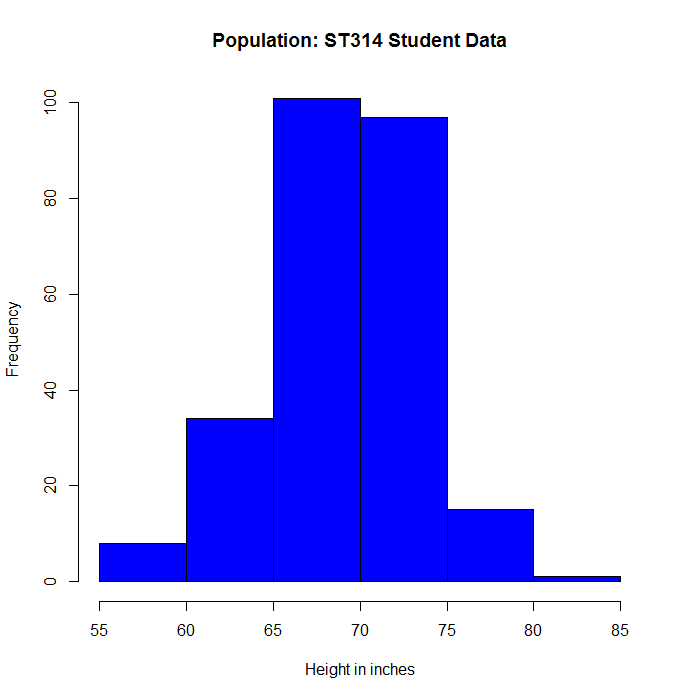
\includegraphics[scale=.5]{student-hist}\\
The majority of the population falls between 65 inches and 75 inches in height.
\subsection*{b}
$\bar{x}=69.036$\\
$s=4.71241$\\
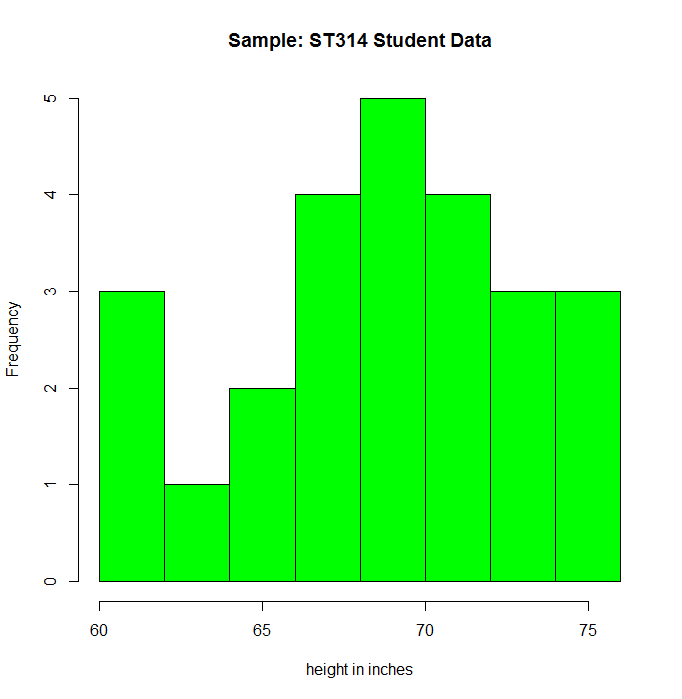
\includegraphics[scale=.5]{sample-student-hist}\\
The sample distribution isn't as radical as the population distribution was.
Most members of the sample lie in the 65-75 range, with some grouping around
60-63. The sample mean was almost exactly the same as the population mean, and
the sample standard deviation was a little bit higher.

\subsection*{c}
$CI=69.036 \pm 1.96*\frac{4.71324}{\sqrt{25}}\\\\
=70.8836$ and $=67.1884$\\\\
The $95\%$ confidence interval for the height of the class is estimated to be
between $67.1884$ and $70.8836$ inches, with a point estimate of $69.036$.
\subsection*{d}
To calculate the t confidence interval for mean height, we do use the following
formua:\\
$CI=\bar{x}\pm t^* * \frac{s}{\sqrt{n}}$\\\\
$69.036 \pm 2.064*\frac{4.71324}{\sqrt{25}}$\\\\
$=70.9816$ and $=67.0904$\\\\
The $95\%$ confidence interval for the height of the sample from class is
estimated to be between $67.0904$ and $70.9816$ inches, with a point estimate
of $69.036$.\\
This interval does include the true population mean of $69.036$.\\

\subsection*{e}
The difference between parts c and d are that, in one, we're taking the CI of
the sample knowing what the population standard deviation is, while in part d,
we're taking the CI without knowing the population SD. The two answers we got
are not too different from each other.

\section*{Part III}
\subsection*{a}
I would anticipate that we would reject the null hypothesis as our sampled
data from our previous measurements had a different mean. The mean
difference was small, but I think it was enough to reject.

\subsection*{b}
To find the t statistic with the formula:\\\\
$t=\frac{\bar{x}-\mu_0}{\frac{s}{\sqrt{n}}}$\\\\
Using the values we found in part II:\\\\
$t=\frac{69.036-69.639}{\frac{4.7124}{\sqrt{256}}}$\\\\
$t=\frac{-.603}{\frac{4.7124}{16}}$\\\\
$t=-2.0474$\\\\
Using this test statistic, we can find our t-value with a $DF=n-1=255$, with a
confidence interval of $95\%$, and a significance level of $.05$. From this 
information, we know that if our p-value (t in this case) is greater than the
degrees of freedom at $95\%$ then we should reject. In this case:\\
$DF=255$\\\\
The value at that value is: $critical(100) < p < critical(1000) = 1.962 < p < 
1.984$\\\\
Knowing this, we can say that in order to reject the null hypothesis, the value
would have to be less than $-1.984$ or greater than $1.984$. We can see that
the value of $-2.0474$ falls outside that range, so we should reject the
null hypothesis.

\subsection*{c}
There is convincing evidence the average height of the students in the
class differ from $69.6393$. The sample estimates the average height to be be 
$69.036$ with a $95\%$ confidence interval of $67.0904$ to $70.9816$ inches. The
null hypothesis is rejected at a significance level of $.05$. The average
height of the students in the class is not $69.6393$ inches.


\section*{Part IV}
\subsection*{a}
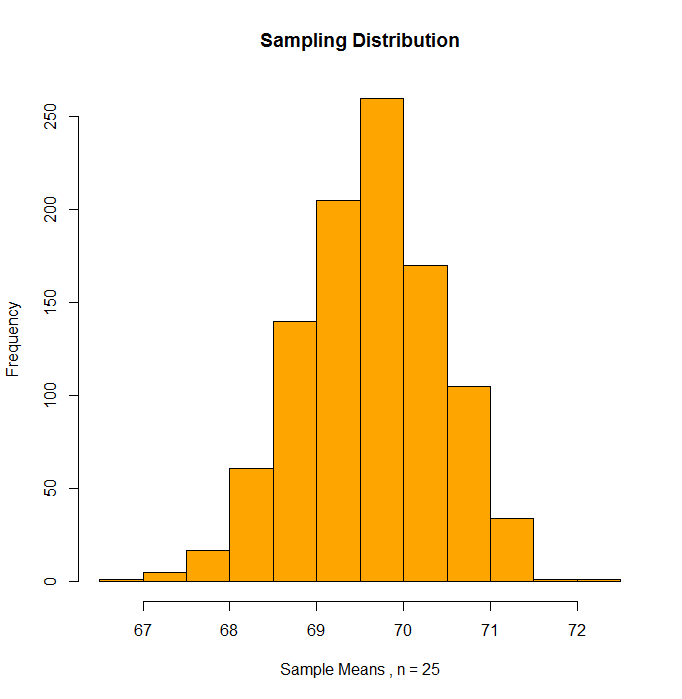
\includegraphics[scale=.5]{sampling}\\
The mean is $69.62365$ and the standard deviation is $.7984$.\\
The central limit theorem states that any sampling distribution of the mean of
any independent, random variable will be normal or nearly normal, if the sample
size is large enough. For our case here, this seems to be the case. The 
distribution is nearly normal.

\subsection*{b}
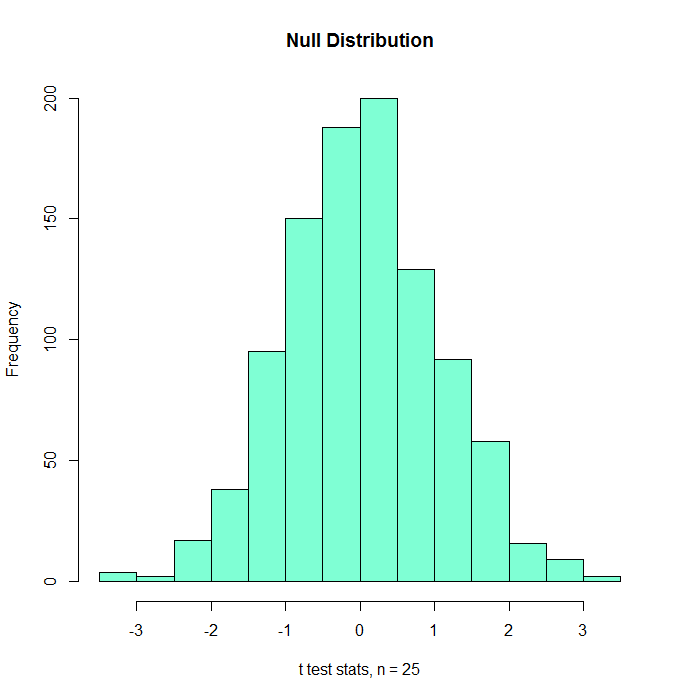
\includegraphics[scale=.5]{null-dist}\\
A normal distribution would model this set of data well. It is nearly normal.

\subsection*{c}
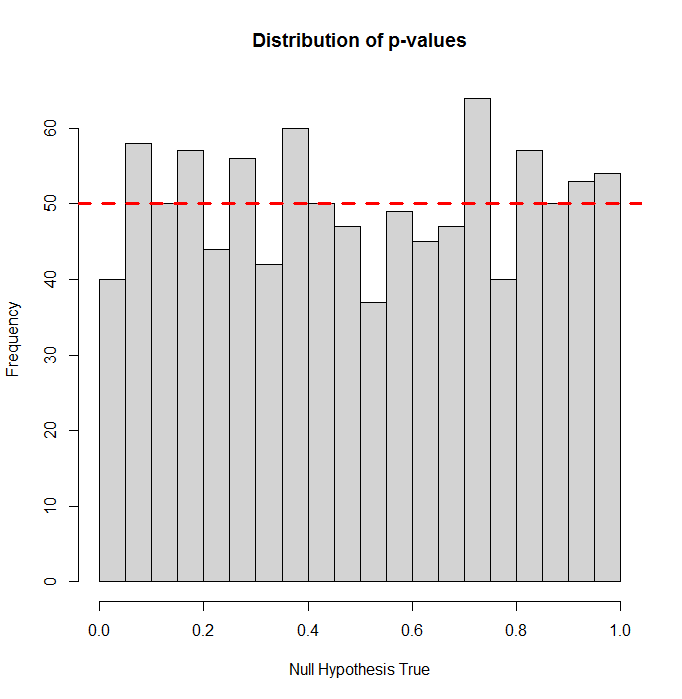
\includegraphics[scale=.5]{p-dist}\\
This does not seem to be the case. The null hypothesis is falsely rejected 
about $4\%$ of the time. This represents type 1 error, which is the incorrect
rejection of true null hypothesis, or a false positive. 

\section*{Part V}
\subsection*{a}
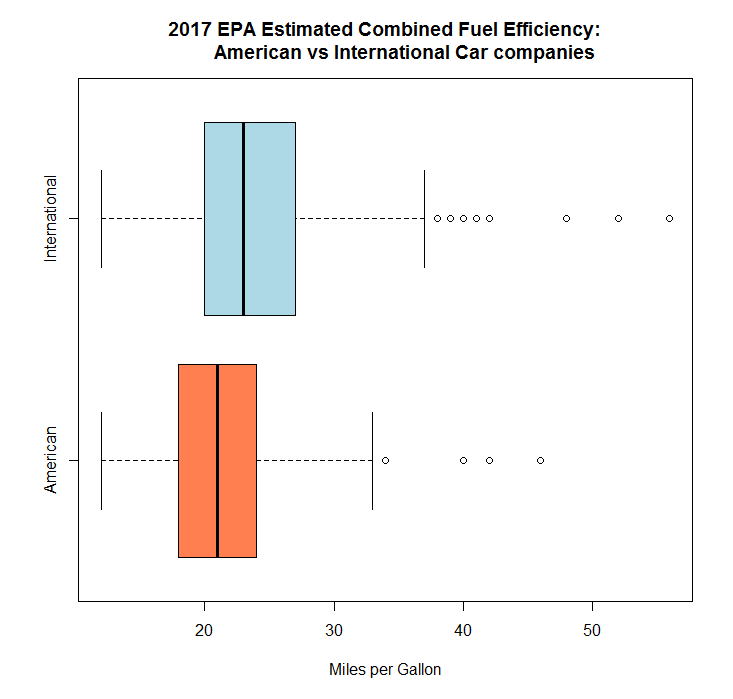
\includegraphics[scale=.5]{fuel-box}\\
There is some visual evidence that the average combined fuel efficiency for the
international car companies is slightly higher than the american average. We can
look at the beginning and ends of the first and third quartiles and see that
the international companies have a slightly higher average value for the
majority of the data points in those ranges.

\subsection*{b}
\begin{center}
	\begin{tabular}{l | c | c | r}
		 & Mean CFE & SD & Sample Size \\
		International & 23.502 & 5.766 & 581 \\
		American & 21.79 & 4.84  & 267
	\end{tabular}
\end{center}
\subsection*{c}
Null Hypothsis: Average CFE American = Average CFE International\\
Alt. Hypothesis: Average CFE American $\neq$ Average CFE International

\subsection*{d}
$n_1$ and $n_2$ are Random Sample: yes\\
Populations and samples are independent: yes, American and International \\
Populations are normal or sample sizes are large: large population size  

\subsection*{e}
To find the test statistic, we can use the formula:\\\\
$t=\frac{\bar{X_1}-\bar{X_2}-(\delta_0)}{\sqrt{\frac{s_1^2}{n_1}+\frac{s_2^2}{n_2}}}$\\\\
$\delta_0=\mu_1 - \mu_2 = (23.502-21.79)-(21.79-23.502)=3.424$\\\\
$\bar{X_1}=23.502$\\
$\bar{X_2}=21.79$\\
$DF=min(n_1 - 1, n_2 - 1)=min(581-1, 267-1)=min(580,266)=266$\\\\
Knowing the above variables, we can plug them in:\\\\
$t=\frac{(23.502-21.79)-(3.424)}{\sqrt{\frac{5.766^2}{581}+\frac{4.84^2}{267}}}$\\\\
$t=-4.496$

\subsection*{f}
Looking up the p-value on the t table, we find that it's less than .001. We
will use this value as it is the one we have.

\subsection*{g}
To find the confidence interval, we use the formula:\\\\
$\bar{X_1}-\bar{X_2}\pm t^*\sqrt{\frac{s_1^2}{n_1}+\frac{s_2^2}{n_2}}$\\\\
$23.502-21.795 \pm .001 * \sqrt{\frac{5.766^2}{581}+\frac{4.84^2}{267}}$\\\\
$=1.71258$ and $1.71182$
Then our confidence interval of 99\% lies between $(1.71192,1.71258)$
\subsection*{h}
They got different confidence interval because they can calculate the exact DF,
we only used the value at 100, the rounded value, and they can also get the
exact p-value, which came out to .000008328 compared to my .001 value.

\subsection*{i}
There is convincing evidence that the average combined fuel efficiency of American
cars versus International have a difference not equal to zero. The sample estimates
the average combined fuel efficiency of International Cars to be 1.71 MPG higher,
with a 99\% confidence interval of $1.71192$ to $1.71258$ MPG. The null hypothesis
is rejected at a significance level of $.01$. The average international car has
a higher average fuel efficiency of about 1.71 MPG. 

There is convincing evidence the average height of the students in the
class differ from $69.6393$. The sample estimates the average height to be be 
$69.036$ with a $95\%$ confidence interval of $67.0904$ to $70.9816$ inches. The
null hypothesis is rejected at a significance level of $.05$. The average
height of the students in the class is not $69.6393$ inches.


\subsection*{j}
There is a practical difference here. About two miles per gallon difference
can add up over a long period. If the difference was much lower, then the value
would be less significant.

\end{document}
